\documentclass[12pt]{article}
\usepackage[utf8]{inputenc}
\usepackage[french]{babel}
\usepackage{amsmath,amsthm,amsfonts,amssymb}
\usepackage{lmodern}
\usepackage[top=2.4cm,bottom=2.4cm,left=2cm,right=2cm]{geometry}
\usepackage{hyperref}
\usepackage{multicol}
\usepackage{enumitem}
\usepackage{listings}
\usepackage[dvipsnames]{xcolor}
\usepackage{tikz}
\date{}
\author{MABROUK Fayez}
\title{{\bf  Génie logiciel} \\
	Rendu de Td \no 10  \\
	{\small L3 Informatique appliquée 2022-2023} \\
	{\it \small \no étudiant : 22213839}}
\begin{document}
	\maketitle
	\newpage
	\section{Auto-portrait, version UML}
Représentez les individus prenant part au cours de Génie Logiciel sous forme de diagramme de
classe. Vous devez d’abord identifier les classes pertinentes, représenter les liens entre ces
différentes classes et enfin renseigner les attributs et les méthodes correspondant à leur rôle.
	\begin{figure}[!hbtp]
	\centering
	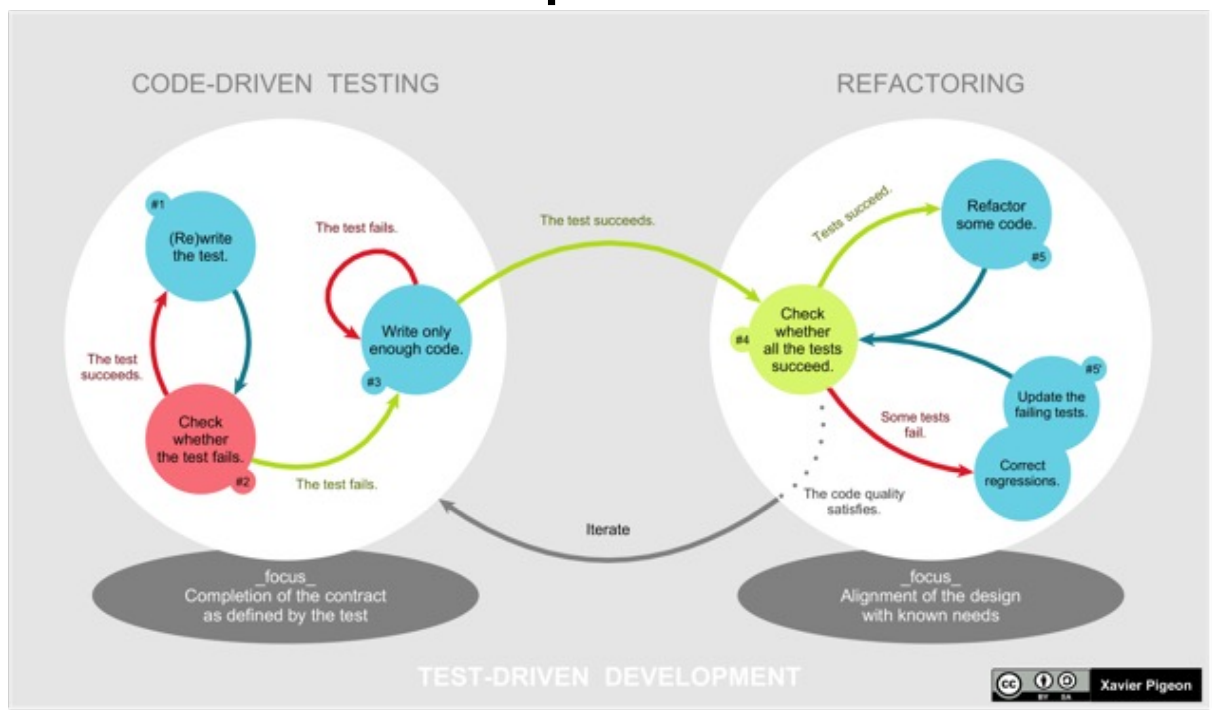
\includegraphics[scale=0.75]{Capture1.png}
	%\caption{Légende de l'image}
\end{figure}
\section{Partie 2 – Bibliothèque}
Nous souhaitons faire un diagramme de classe pour l’exemple de la bibliothèque étudié lors des
semaines précédentes.
\begin{itemize}
	\item[1. ] Représentez les différentes classes du système. Vous réfléchirez en particulier sur la
	nécessité éventuelle d’ajouter des classes n’apparaissant pas sur vos précédents diagrammes
	de ce modèle (cas d’utilisation, séquence). On fera la différence entre un emprunteur
	étudiant (peut emprunter 5 livres à la fois), et un personnel de l’université (pouvant
	emprunter 10 livres à la fois).
	\item[2. ] Représentez les liens entre ces classes.
	\item[3. ] Ajoutez les attributs et méthodes de chacune des classes.\\
	\\

	
		\begin{figure}[!hbtp]
		\centering
		\includegraphics[scale=0.62]{Capture2_s.png}
		%\caption{Légende de l'image}
	\end{figure}

\end{itemize}
		
	En plus du diagramme, vous devez écrire un petit paragraphe (5-10 lignes) de réflexion sur les
	différentes étapes de modélisation sur l’exemple de la bibliothèque. En particulier, vous devez
	répondre aux questions suivantes : auriez-vous fait le modèle dans cet ordre ? Quelle est la
	complexité de votre modèle ? Est-ce qu’il manque des informations ?\\
	 \\

	 
	$\Rightarrow$ Non, je n’aurais pas fait le modèle de cet ordre parce que je pense que les diagrammes de 
	classes sont plus simples à faire que les diagrammes de séquence, donc pour moi, l’ordre 
	logique c’est Use Case, Classe, Séquence.\\
	Je pense que le modèle, qu’on a fait, est relativement simple et que si quelqu’un, qui ne fait 
	 pas de cours de GL, essaye de le comprendre, il peut facilement.\\
	 Oui, il y a un manque d’informations au niveau des objets eux-mêmes car même si on a fait 
	 les diagrammes de classes, le concept des objets reste très général.
\end{document}